目前为止,本章已经介绍了理解内存模型所需的概念。本章的其余部分详细解释了内存模型,包括\par

\begin{enumerate}
	\item 如何表达内核的内存序要求
	\item 如何查询指定设备支持的内存
	\item 内存模型如何对待不相交的地址空间和多个设备
	\item 内存模型如何与计算栅栏、内存栅栏和原子交互
	\item 缓冲区和USM之间使用原子操作有何不同
\end{enumerate}

内存模型是基于标准C++的内存模型,但在一些重要方面有所不同。这些差异反映了我们的长期愿景,即DPC++和SYCL应该有助于预告未来的C++标准:类的默认行为和命名与C++标准库紧密一致,目的是扩展标准C++功能,而不是限制它。\par

图19-9中的表格总结了在标准C++(C++11, C++14, C++17, C++20)与SYCL和DCP++中不同的内存模型概念是如何作为语言特性使用的。 C++14, C++17和C++20标准还包括了一些对C++实现影响的说明。这些说明不应该影响程序代码,所以这里不讨论它们。\par

\hspace*{\fill} \par %插入空行
图19-9 比较标准C++和SYCL/DPC++内存模型
\begin{center}
	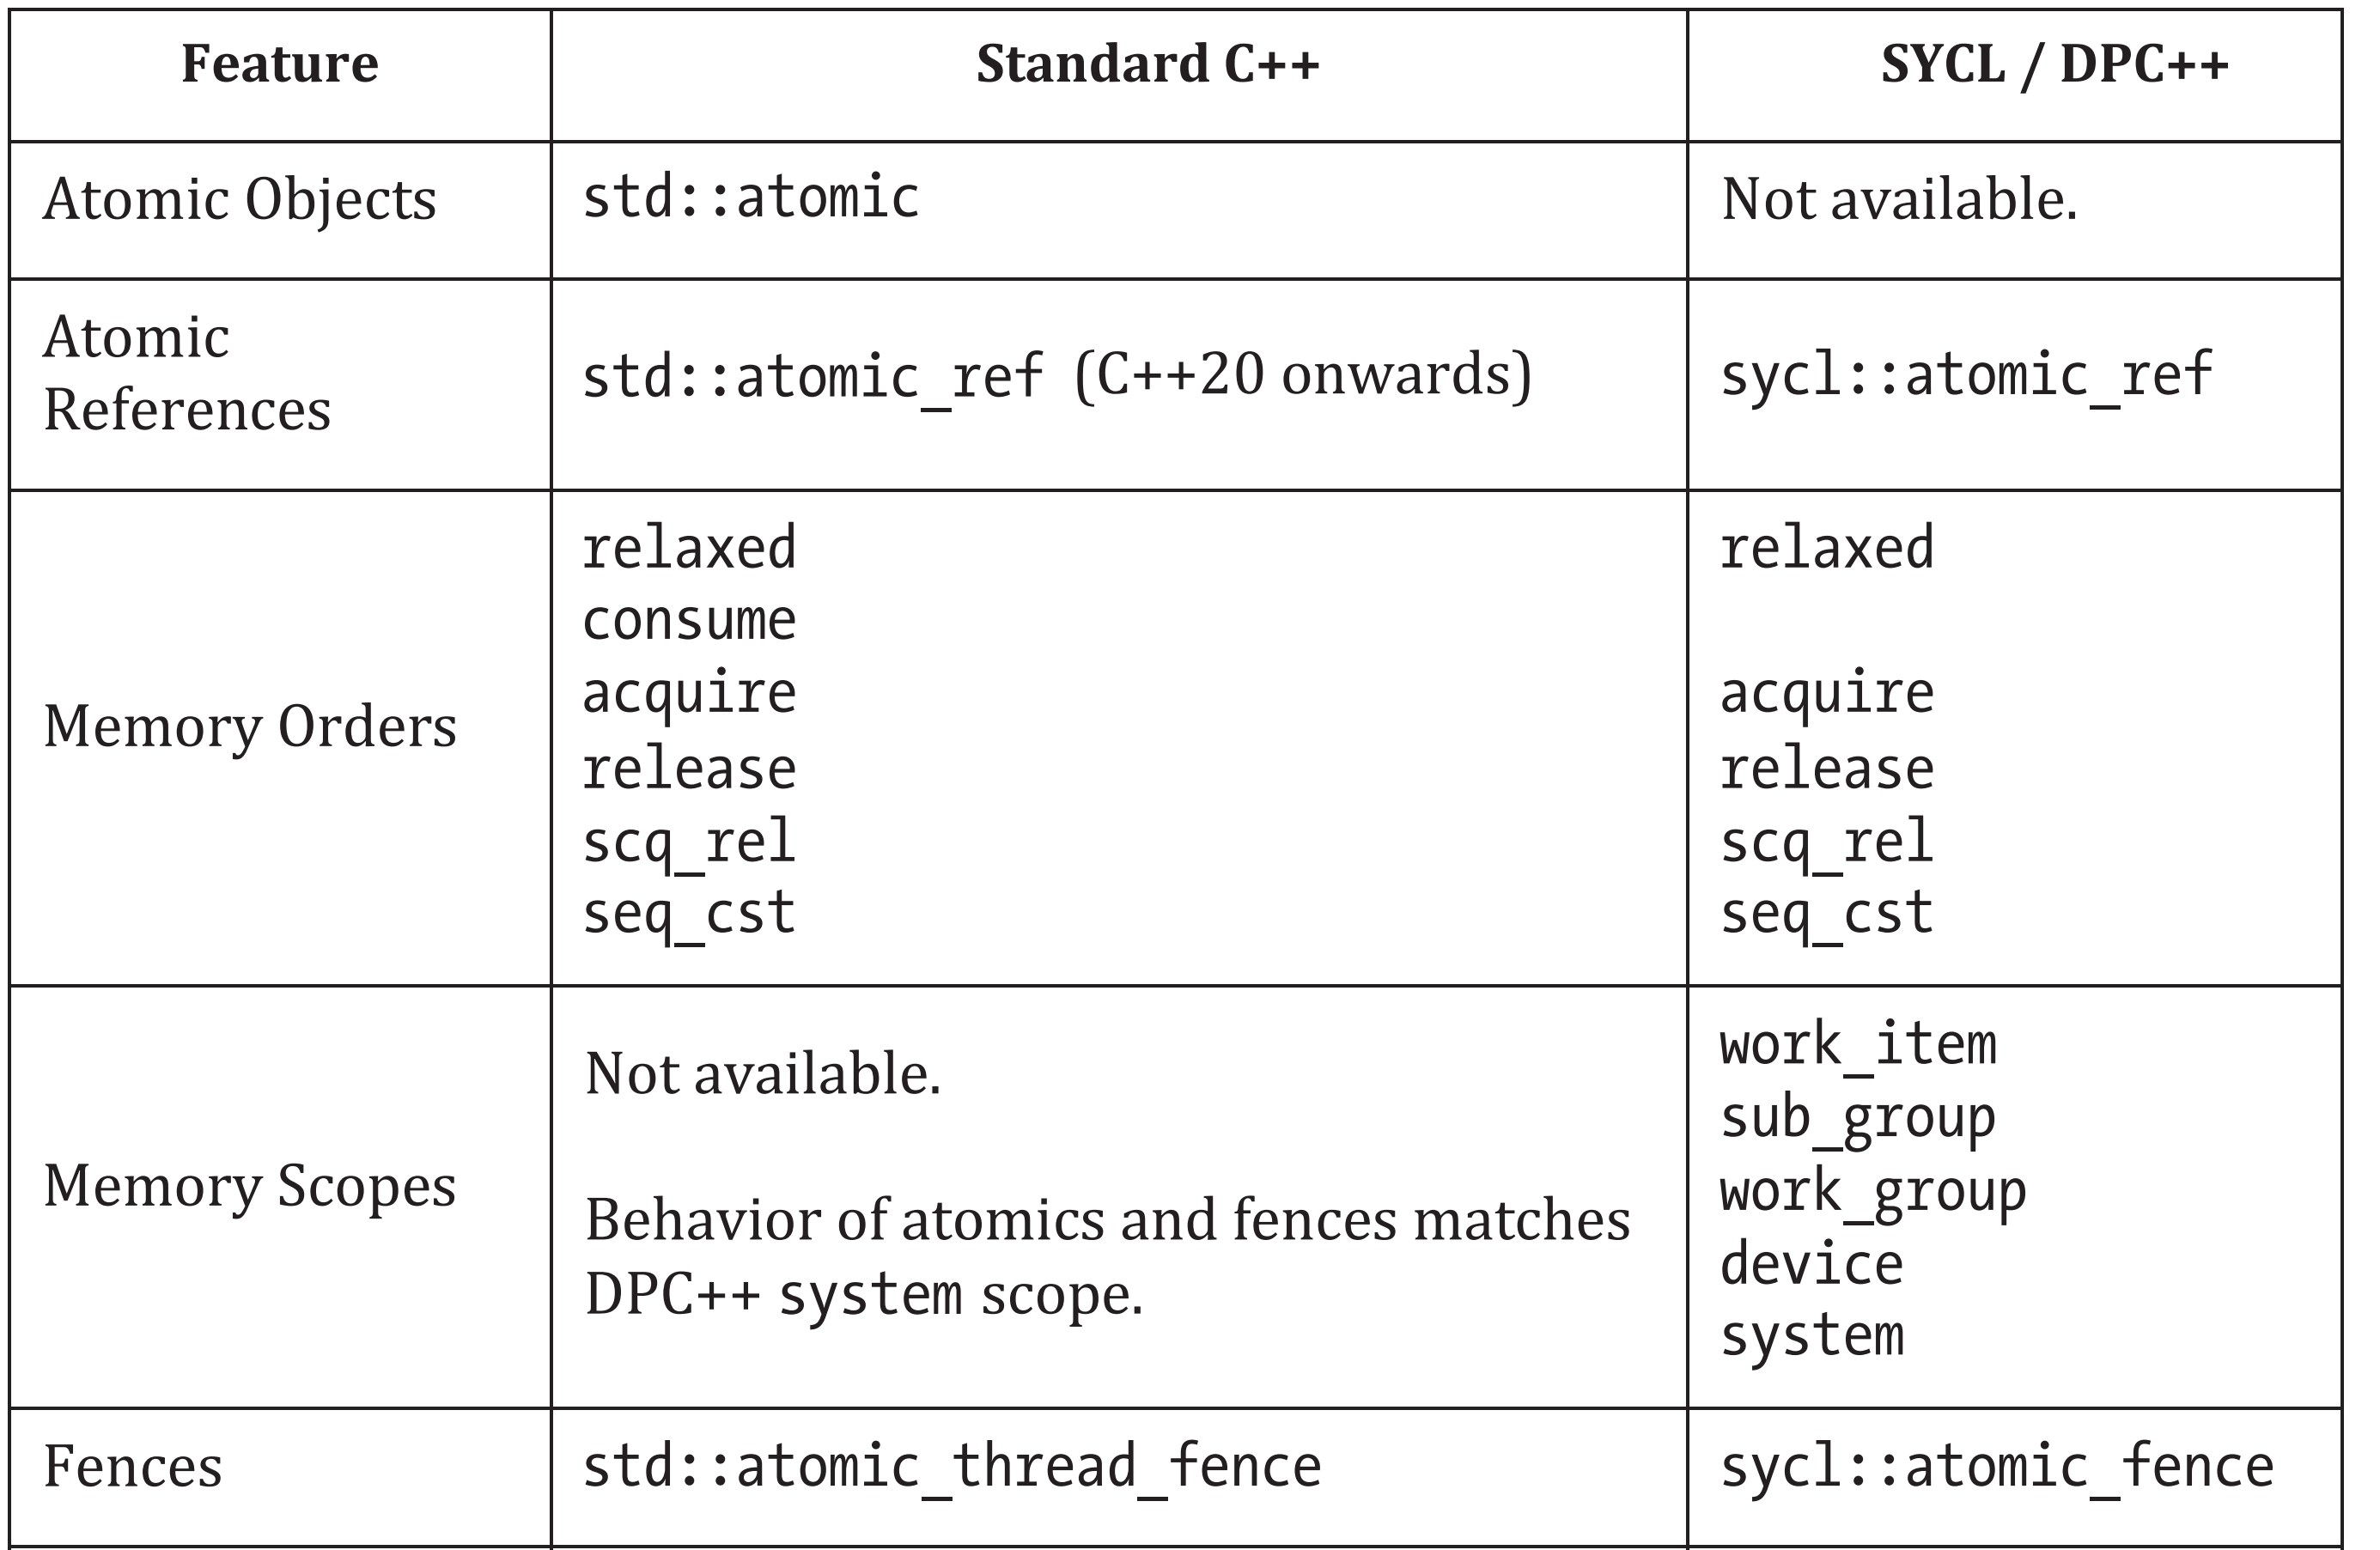
\includegraphics[width=1.0\textwidth]{content/chapter-19/images/6}
	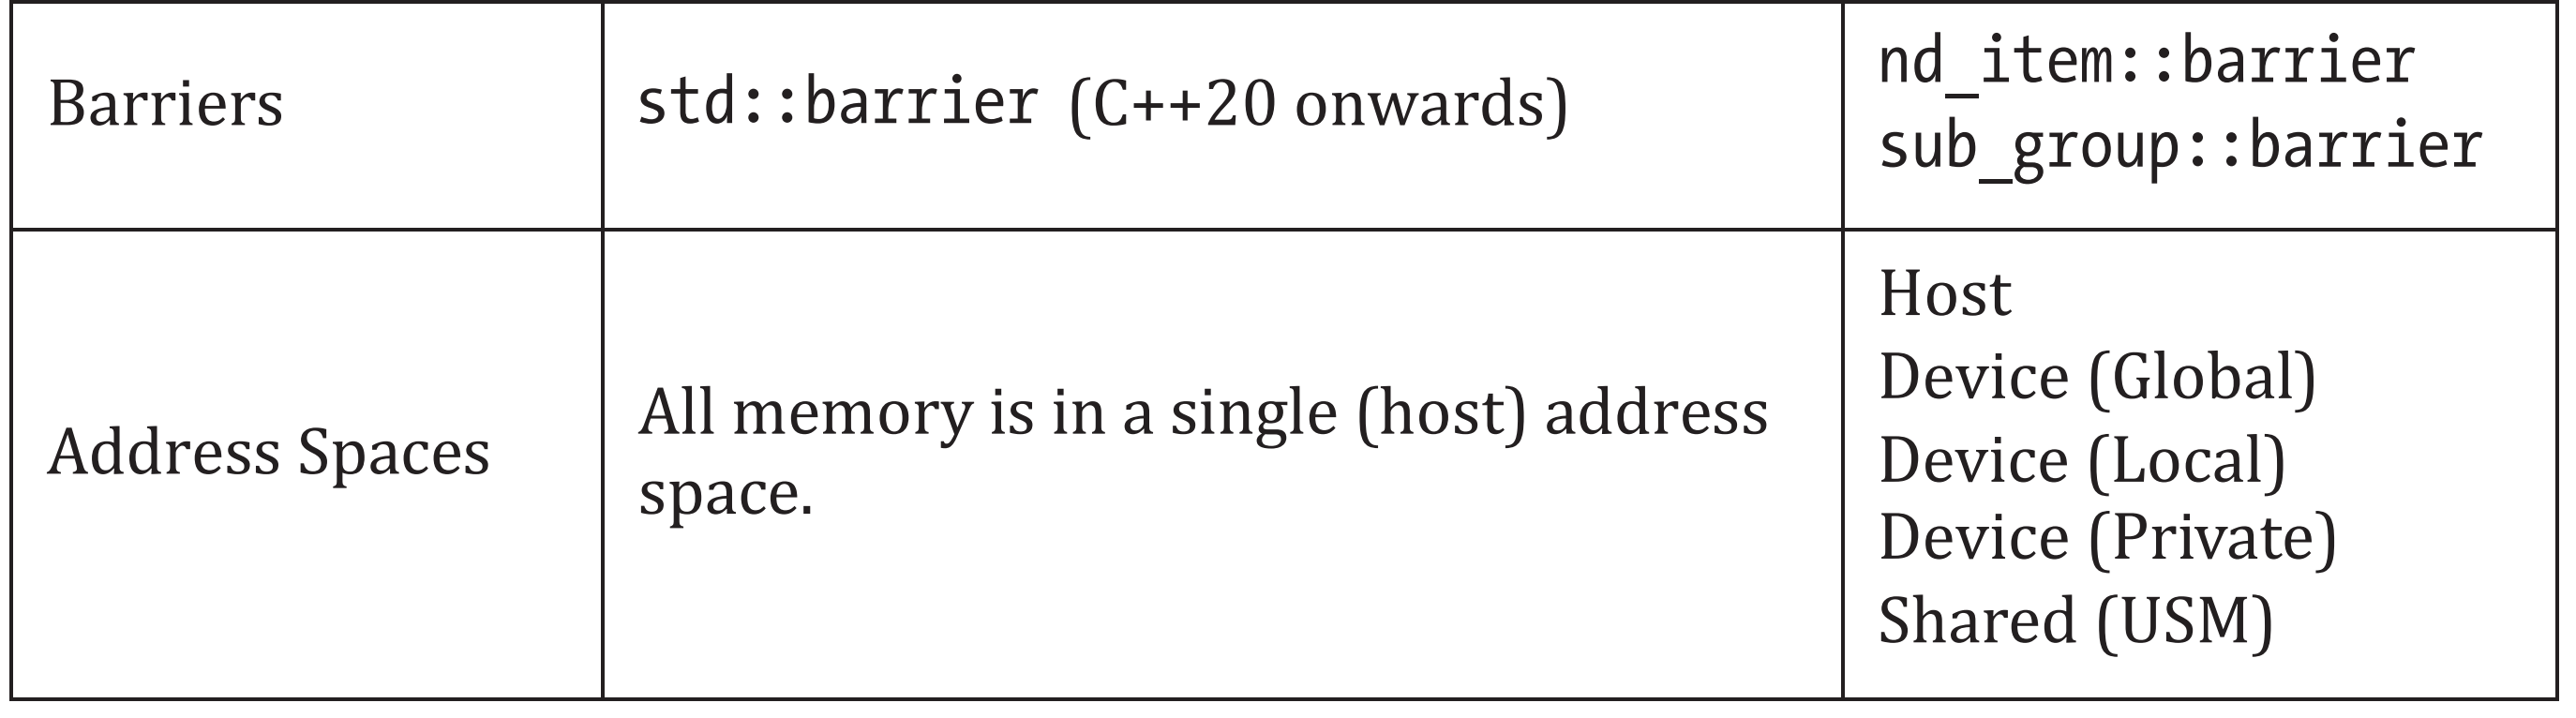
\includegraphics[width=1.0\textwidth]{content/chapter-19/images/7}
\end{center}

\hspace*{\fill} \par %插入空行
\textbf{memory\_order枚举类}

内存模型通过memory\_order枚举类的6个值表示不同的内存序,这些值可以作为参数提供给内存栅栏和原子操作。为一个操作提供一个内存序参数,告诉编译器相对于该操作的所有其他内存操作(任何地址)需要以什么内存序,如下所述:\par

\begin{itemize}
	\item memory\_order::relaxed \\
	读写操作可以在操作之前或之后重排,没有任何限制。没有顺序保证。
	\item memory\_order::acquire \\
	操作之后出现的读和写操作必须在该操作之后出现(也就是说,不能在操作之前重排)。
	\item memory\_order::release \\ 
	操作之前出现的读操作和写操作必须在程序的操作之前发生(即,不能在操作之后重排),并且前面的写操作保证对其他程序实例可见,这些程序实例已经通过相应的获取操作(即,使用相同的变量和memory\_order::acquire或barrier函数的原子操作)。
	\item memory\_order::acq\_rel \\
	操作既是获取也是释放。读和写操作不能围绕操作重排,前面的写操作必须像前面描述的memory\_order::release一样可见。
	\item memory\_order::seq\_cst \\
	该操作分别作为获取、释放或两者都起作用,具体取决于它是读操作、写操作或读-改-写操作。以顺序一致的内存序执行操作。
\end{itemize}

对于每个操作所支持的内存顺序有几个限制。图19-10中的表格总结了有效的组合。\par

\hspace*{\fill} \par %插入空行
图19-10 使用memory\_order支持原子操作
\begin{center}
	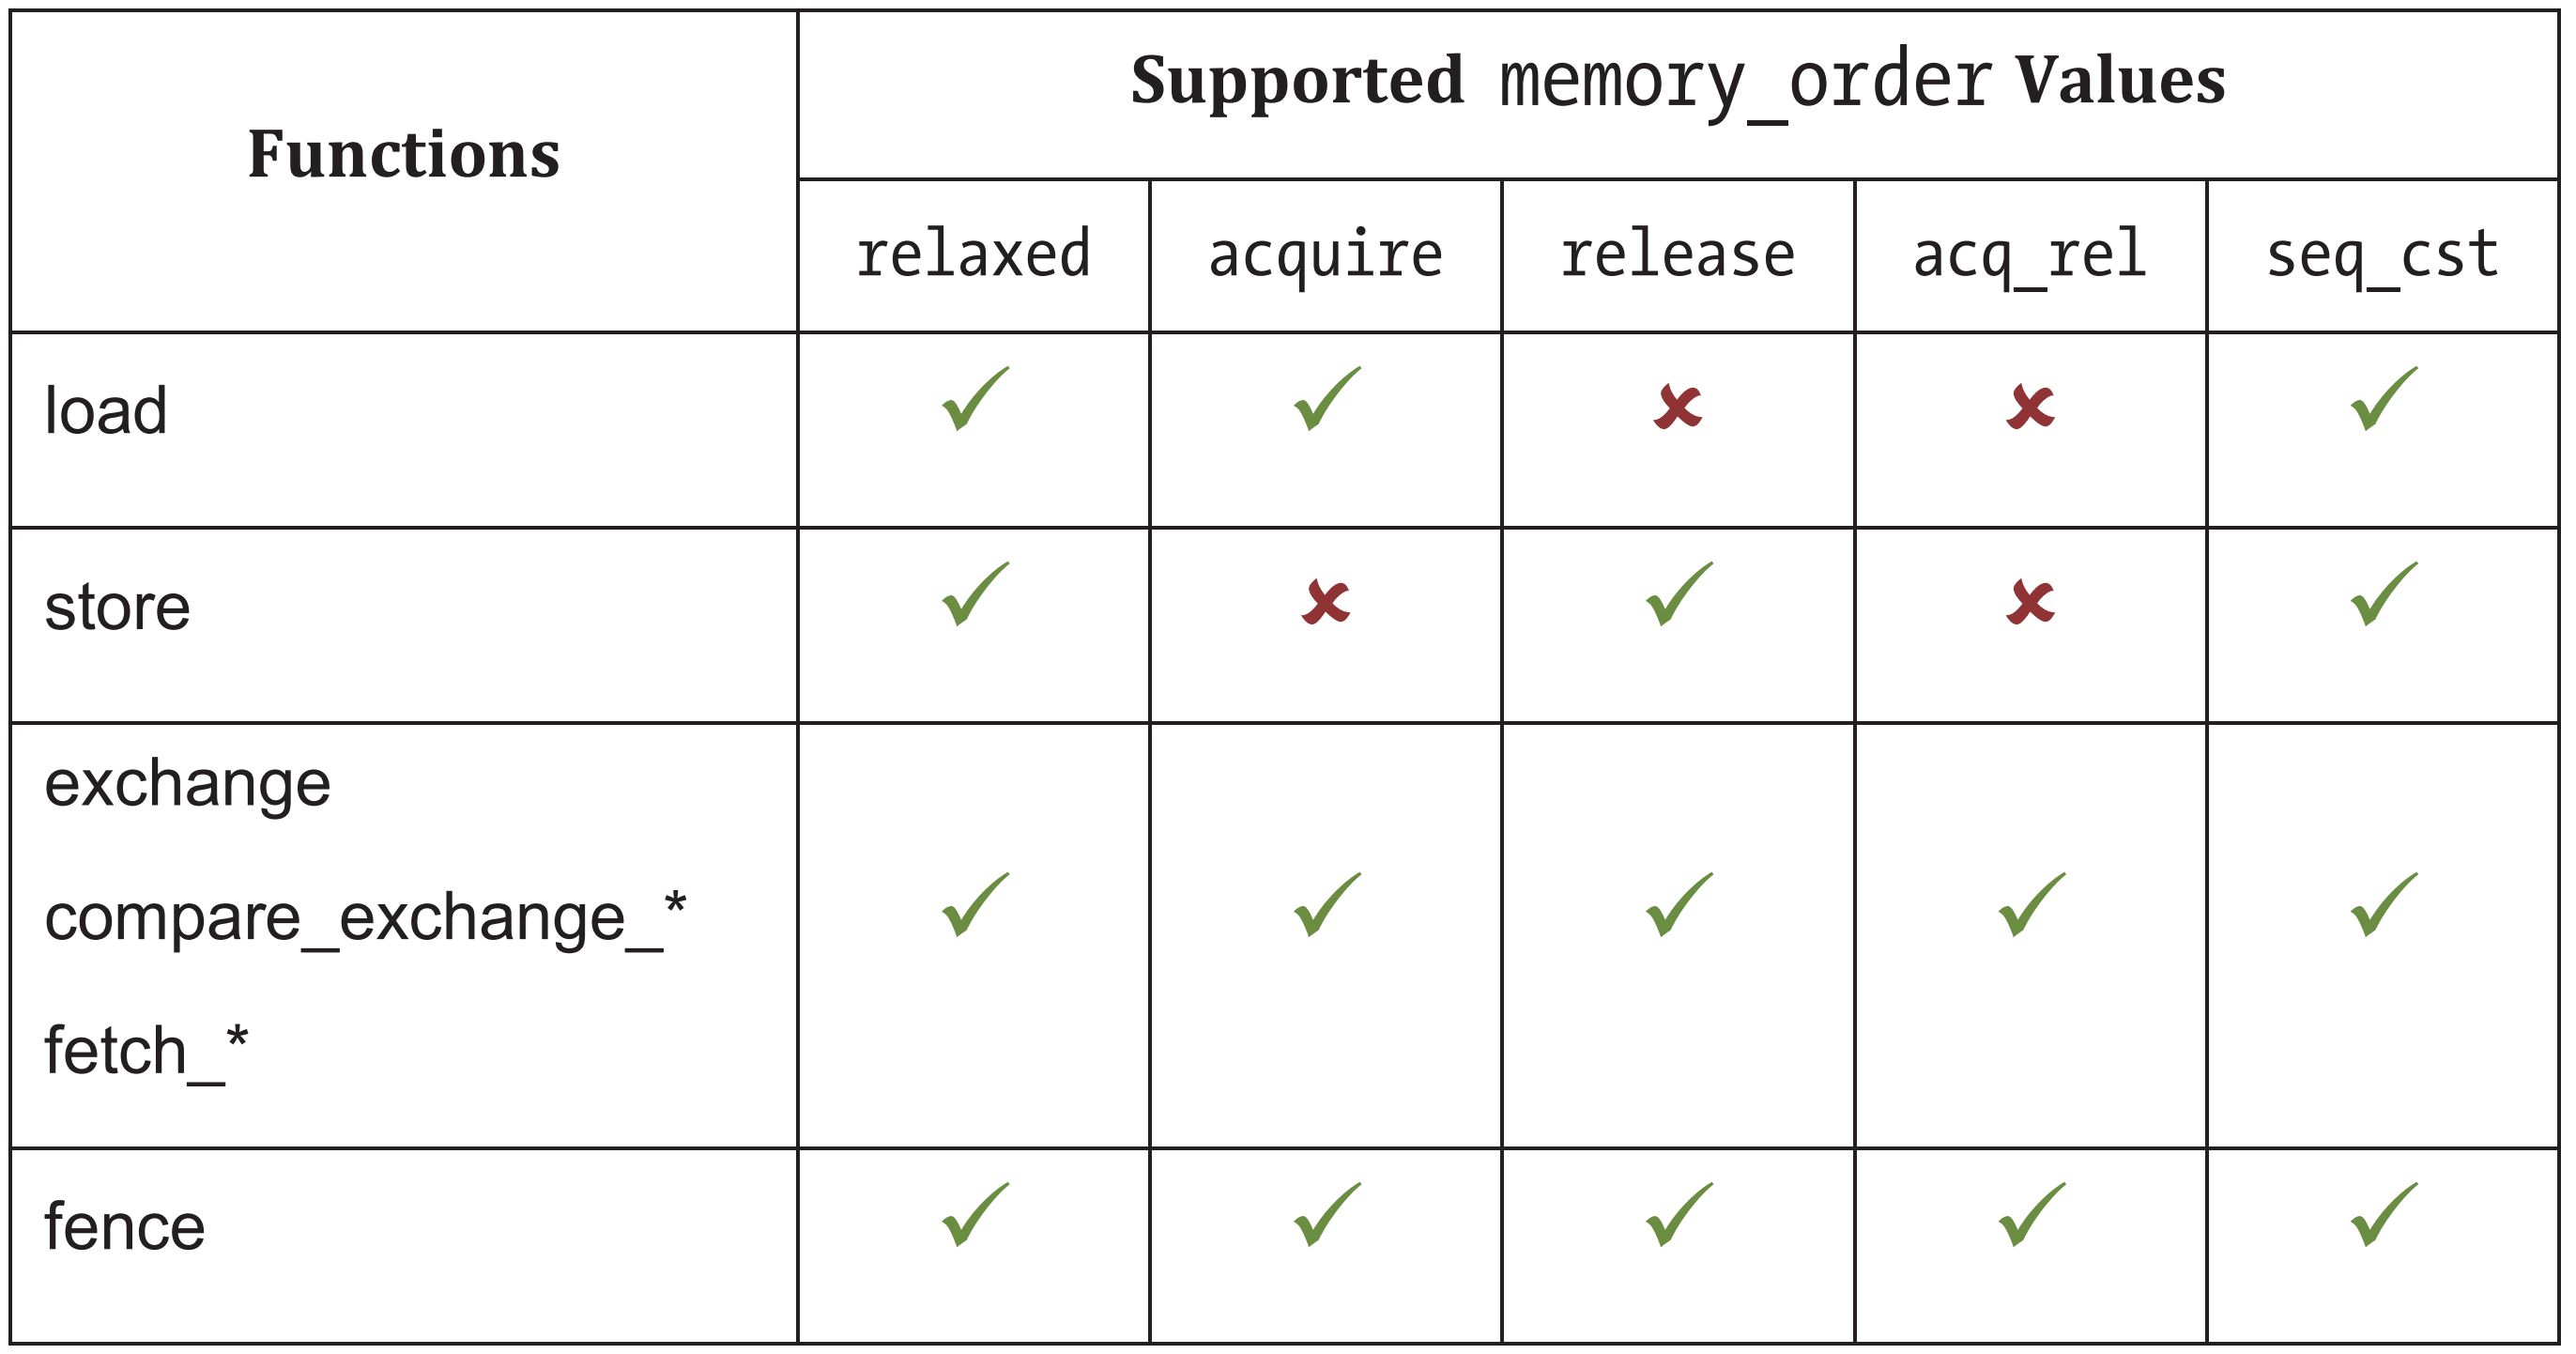
\includegraphics[width=1.0\textwidth]{content/chapter-19/images/8}
\end{center}

加载操作不会将值写入内存,因此与释放语义不兼容。类似地,存储操作不从内存中读取值,因此与获取语义不兼容。其余的读-改-写原子操作和内存栅栏与所有内存序兼容。\par

\begin{tcolorbox}[colback=blue!5!white,colframe=blue!75!black, title=C++中的内存序]
C++内存模型还包括memory\_order::consume,其行为与memory\_order::acquire类似。然而,C++17标准不鼓励使用它,注意到它的定义正在修订。它在DPC++中的实现会推迟到未来的版本。
\end{tcolorbox}

\hspace*{\fill} \par %插入空行
\textbf{memory\_scope枚举类}

标准的C++内存模型假设应用程序,在具有单个地址空间的单个设备上执行。这两种假设都不适用于DPC++应用程序:应用程序的不同部分在不同的设备上执行(例如,一个主机设备和一个或多个加速器设备);每个设备有多个地址空间(即,私有,本地和全局);并且每个设备的全局地址空间可能是是断开的(取决于USM支持)。\par

为了解决这个问题,DPC++扩展了C++内存顺序的概念,以包括原子操作的范围,表示给定内存顺序约束应用的最小工作集。作用域集合是通过memory\_scope枚举类定义的:\par

\begin{itemize}
	\item memory\_scope::work\_item \\
	内存序约束仅应用于调用工作项。这个作用域只对映像操作有用,因为工作项中的所有其他操作已经保证按程序顺序执行。
	\item memory\_scope::sub\_group, memory\_scope::work\_
	group \\
	内存序约束仅应用于与调用工作项相同的子工作组或工作组中的工作项。
	\item memory\_scope::device \\ 
	内存序约束仅适用于在与调用工作项相同的设备上执行的工作项。
	\item memory\_scope::system \\
	内存排序约束适用于系统中的所有工作项。
\end{itemize}

除了设备功能所施加的限制,所有内存作用域都是所有原子操作和内存栅栏操作的有效参数。但在以下三种情况之一中,作用域参数可能会自动降级为较窄的作用域:\par

\begin{enumerate}
	\item 当原子操作更新了工作组本地内存中的值,则任何比memory\_scope::work\_group范围更宽的作用域都会缩小(因为本地内存只对同一个工作组中的工作项可见)。
	\item 当设备不支持USM,指定memory\_scope::system等同于memory\_scope::device(因为缓冲区不能被多个设备同时访问)。
	\item 当原子操作使用memory\_order::relaxed,则没有顺序保证,并且内存作用域参数会被忽略。
\end{enumerate}

\hspace*{\fill} \par %插入空行
\textbf{查询设备能力}

为了确保与SYCL以前版本支持的设备的兼容性,并最大化可移植性,DPC++支持OpenCL 1.2设备和其他可能无法支持完整C++内存模型的硬件(例如,某些类型的嵌入式设备)。DPC++提供设备查询来帮助我们推断系统中,可用设备支持的内存序和内存范围:\par

\begin{itemize}
	\item atomic\_memory\_order\_capabilities \\
	atomic\_fence\_order\_capabilities \\
	返回特定设备上原子操作和内存栅栏操作支持的所有内存序列表。所有设备都必须支持memory\_order::relaxed,并且主机设备必须支持所有内存序。
	\item atomic\_memory\_scope\_capabilities \\
	atomic\_fence\_scope\_capabilities \\
	返回特定设备上原子操作和fence操作支持的所有内存作用域的列表。所有设备都必须至少支持memory\_order::work\_group,并且主机设备必须支持所有内存作用域。
\end{itemize}

一开始可能很难记住哪些内存顺序和作用域支持哪些功能和设备功能的组合。在实践中,可以通过以下两种开发方法来避免这种复杂性:\par

\begin{enumerate}
	\item 开发具有顺序一致性和系统栅栏的应用程序。\\
	性能调优期间,只考虑采用不那么严格的内存序。
	\item 开发具有自由一致性和工作组栅栏的应用程序。 \\
	只有在需要正确性时,才考虑采用更严格的内存序和更广泛的作用域。
\end{enumerate}

第一种方法确保所有原子操作和栅栏语义匹配标准C++的默认行为。这是最简单、最不容易出错的选项,但是具有性能和可移植性最差的特征。\par

第二种方法更符合SYCL以前版本和OpenCL等语言的默认行为。虽然更复杂——因为它要求我们更加熟悉不同的内存序和作用域——确保我们编写的大部分DPC++代码可以在任何设备上运行,而不会造成性能损失。\par

\hspace*{\fill} \par %插入空行
\textbf{栅栏}

目前为止,本书中所有之前使用的栅栏都忽略了内存序和作用域的问题,而是依赖于默认行为。\par

DPC++中的每一个工作组栅栏对于调用工作项可访问的所有地址空间都起到了获取-释放的作用,并且使得前面的写操作至少对同一组中的所有其他工作项可见。这确保了一组工作项在栅栏之后的内存一致性,这与我们对同步的直观理解(以及同步的定义——与C++中的关系)一致。\par

atomic\_fence函数提供了比这更细粒度的控制,允许工作项以指定的内存顺序和范围执行栅栏。DPC++的未来版本中,工作组栅栏可能同样接受一个可选参数来调整与栅栏相关的获取-释放栅栏的内存作用域\par

\hspace*{\fill} \par %插入空行
\textbf{DPC++中的原子操作}

DPC++支持对各种数据类型的多种原子操作。所有设备都保证支持通用操作(例如,加载、存储、算术操作符)的原子版本,以及实现无锁算法所需的原子比较和交换操作。该语言为所有基本整数、浮点数和指针类型定义了这些操作——所有设备都必须支持32位类型的这些操作,但64位类型的支持是可选的。\par

\hspace*{\fill} \par %插入空行
\textbf{atomic类}

C++11中的std::atomic类提供了一个创建和操作原子变量的接口。原子类的实例拥有数据,不能移动或复制,只能使用原子操作进行更新。这些限制大大减少了不正确使用类和引入未定义行为的机会。它们也阻止了类在DPC++内核中使用——在主机上创建原子对象并将它们传输到设备上是不可能的!我们可以在宿主代码中继续使用std::atomic,但是尝试在设备内核中使用将导致编译错误。\par

\begin{tcolorbox}[colback=blue!5!white,colframe=blue!75!black, title=原子类在SYCL 2020和DPC++中已弃用]
SYCL 1.2.1规范包括一个cl::sycl::atomic类,它基于C++11中的std::atomic类。这两个类的接口有一些不同,最值得注意的是SYCL 1.2.1版本不拥有自己的数据,默认情况下使用宽松的内存序。\\

DPC++完全支持cl::sycl::atomic类,但是为了避免混淆,不建议使用它。我们建议使用atomic\_ref类(将在下一节中讨论)代替它。
\end{tcolorbox}

\hspace*{\fill} \par %插入空行
\textbf{atomic\_ref类}

C++20中的std::atomic\_ref类为原子操作提供了一个替代接口,它比std::atomic提供了更大的灵活性。这两个类之间最大的区别是std::atomic\_ref的实例并不拥有数据,而是从现有的非原子变量构造而来。创建原子引用实际上相当于一个承诺,即引用的变量只在引用的生命周期内进行原子访问。这些正是DPC++所需要的语义,因为它们允许在主机上创建非原子数据,将数据传输到设备,并且只有在它传输之后才将其视为原子数据。因此,DPC++内核中使用的atomic\_ref类是基于std::atomic\_ref的。\par

我们说基于,因为类的DPC++版本包括三个额外的模板参数,如图19-11所示。\par

\hspace*{\fill} \par %插入空行
图19-11 atomic\_ref类的构造函数和静态成员
\begin{lstlisting}[caption={}]
template <typename T,
			memory_order DefaultOrder,
			memory_scope DefaultScope, 
			access::address_space AddressSpace>
class atomic_ref {
public:
	using value_type = T;
	static constexpr size_t required_alignment =
		/* implementation-defined */;
	static constexpr bool is_always_lock_free =
		/* implementation-defined */;
	static constexpr memory_order default_read_order =
		memory_order_traits<DefaultOrder>::read_order;
	static constexpr memory_order default_write_order =
		memory_order_traits<DefaultOrder>::write_order;
	static constexpr memory_order default_read_modify_write_order =
		DefaultOrder;
	static constexpr memory_scope default_scope = DefaultScope;
	
	explicit atomic_ref(T& obj);
	atomic_ref(const atomic_ref& ref) noexcept;
};
\end{lstlisting}

正如前面所讨论的,不同DPC++设备的功能是不同的。为DPC++的原子类选择一个默认行为比较困难:默认为标准C++行为(即,memory\_order::seq\_cst,memory\_scope::system)限制代码只能在最有能力的设备上执行;另一方面,在迁移现有C++代码时,打破C++约定并默认使用最小公分母(即memory\_order::relaxed, memory\_scope::work\_group)可能会导致意外行为。DPC++采用的设计提供了一种折中方案,允许我们将所需的默认行为定义为对象类型的一部分(使用DefaultOrder和DefaultScope模板参数)。其他排序和作用域可以作为运行时参数提供给特定的原子操作——DefaultOrder和DefaultScope只影响那些没有或不能覆盖默认行为的操作(例如,当使用像+=这样的简写操作符时)。模板的最后一个参数表示被引用对象分配的地址空间。\par

原子引用根据所引用对象的类型为不同的操作提供支持。所有类型支持的基本操作如图19-12所示,提供了原子地将数据移动到内存和从内存中移动数据的能力。\par

\hspace*{\fill} \par %插入空行
图19-12。使用atomic\_ref对所有类型进行操作
\begin{lstlisting}[caption={}]
void store(T operand,
	memory_order order = default_write_order,
	memory_scope scope = default_scope) const noexcept;
T operator=(T desired) const noexcept; // equivalent to store

T load(memory_order order = default_read_order,
	memory_scope scope = default_scope) const noexcept;
operator T() const noexcept; // equivalent to load

T exchange(T operand,
	memory_order order = default_read_modify_write_order,
	memory_scope scope = default_scope) const noexcept;
	
bool compare_exchange_weak(T &expected, T desired,
	memory_order success,
	memory_order failure,
	memory_scope scope = default_scope) const noexcept;
	
bool compare_exchange_weak(T &expected, T desired,
	memory_order order = default_read_modify_write_order,
	memory_scope scope = default_scope) const noexcept;
	
bool compare_exchange_strong(T &expected, T desired,
	memory_order success,
	memory_order failure,
	memory_scope scope = default_scope) const noexcept;
	
bool compare_exchange_strong(T &expected, T desired,
	memory_order order = default_read_modify_write_order,
	memory_scope scope = default_scope) const noexcept;
\end{lstlisting}

对整数和浮点类型对象的原子引用扩展了可用原子操作集,以包括算术操作,如图19-13和19-14所示。设备必须支持原子浮点类型,不管是否具有对硬件中浮点原子的支持,而且许多设备都希望使用原子比较交换来模拟原子浮点加法。这种模拟是DPC++中提供性能和可移植性的重要部分,可以自由地在算法需要的地方使用浮点原子——结果代码将正确工作,并将受益于浮点原子硬件的改进而无需任何修改!\par

\hspace*{\fill} \par %插入空行
图19-13 仅对整数类型使用atomic\_ref的附加操作
\begin{lstlisting}[caption={}]
Integral fetch_add(Integral operand,
	memory_order order = default_read_modify_write_order,
	memory_scope scope = default_scope) const noexcept;
	
Integral fetch_sub(Integral operand,
	memory_order order = default_read_modify_write_order,
	memory_scope scope = default_scope) const noexcept;
	
Integral fetch_and(Integral operand,
	memory_order order = default_read_modify_write_order,
	memory_scope scope = default_scope) const noexcept;
	
Integral fetch_or(Integral operand,
	memory_order order = default_read_modify_write_order,
	memory_scope scope = default_scope) const noexcept;
	
Integral fetch_min(Integral operand,
	memory_order order = default_read_modify_write_order,
	memory_scope scope = default_scope) const noexcept;

Integral fetch_max(Integral operand,
	memory_order order = default_read_modify_write_order,
	memory_scope scope = default_scope) const noexcept;

Integral operator++(int) const noexcept;
Integral operator--(int) const noexcept;
Integral operator++() const noexcept;
Integral operator--() const noexcept;
Integral operator+=(Integral) const noexcept;
Integral operator-=(Integral) const noexcept;
Integral operator&=(Integral) const noexcept;
Integral operator|=(Integral) const noexcept;
Integral operator^=(Integral) const noexcept;
\end{lstlisting}

\hspace*{\fill} \par %插入空行
图196-4 仅用于浮点类型的atomic\_ref的附加操作
\begin{lstlisting}[caption={}]
Floating fetch_add(Floating operand,
	memory_order order = default_read_modify_write_order,
	memory_scope scope = default_scope) const noexcept;
	
Floating fetch_sub(Floating operand,
	memory_order order = default_read_modify_write_order,
	memory_scope scope = default_scope) const noexcept;
	
Floating fetch_min(Floating operand,
	memory_order order = default_read_modify_write_order,
	memory_scope scope = default_scope) const noexcept;
	
Floating fetch_max(Floating operand,
	memory_order order = default_read_modify_write_order,
	memory_scope scope = default_scope) const noexcept;
	
Floating operator+=(Floating) const noexcept;
Floating operator-=(Floating) const noexcept;
\end{lstlisting}

\hspace*{\fill} \par %插入空行
\textbf{缓冲区中使用原子操作}

如上一节所讨论的,在DPC++中没有办法分配原子数据,也不能在主机和设备之间移动。将原子操作与缓冲区结合使用,必须创建非原子数据缓冲区,以便将其传输到设备,然后通过原子引用访问该数据。\par

\hspace*{\fill} \par %插入空行
图19-15 通过显式创建的atomic\_ref访问缓冲区
\begin{lstlisting}[caption={}]
Q.submit([&](handler& h) {
	accessor acc{buf, h};
	h.parallel_for(N, [=](id<1> i) {
		int j = i % M;
		atomic_ref<int, memory_order::relaxed, memory_scope::system,
				access::address_space::global_space> atomic_acc(acc[j]);
		atomic_acc += 1;
	});
});
\end{lstlisting}

图19-15中的代码是在DPC++中使用显式创建的原子引用对象表示原子性的示例。缓冲区存储普通整数,需要具有读和写权限的访问器。然后,可以为每个数据访问创建atomic\_ref实例,使用+=操作符作为fetch\_add成员函数进行替代。\par

如果想在同一个内核中混合对缓冲区的原子和非原子访问,这个模式是有用的,以避免在不需要原子操作时产生性能开销。如果已知缓冲区中只有一个内存位置的子集将被多个工作项并发访问,那么只需要在访问那个子集时使用原子引用即可。或者,如果已知同一个工作组中的工作项仅在内核的一个阶段(即两个工作组栅栏之间)同时访问本地内存,那么只需要在该阶段使用原子引用。\par

有时,我们很乐意为每个访问支付原子性的开销,要么是因为为了正确性,要么是因为关心生产力而不是性能。对于这种情况,DPC++为声明访问器必须始终使用原子操作提供了一种简写,如图19-16所示。\par

\hspace*{\fill} \par %插入空行
图19-16 通过原子访问器隐式创建的atomic\_ref访问缓冲区
\begin{lstlisting}[caption={}]
buffer buf(data);

Q.submit([&](handler& h) {
	atomic_accessor acc(buf, h, relaxed_order, system_scope);
	h.parallel_for(N, [=](id<1> i) {
		int j = i % M;
		acc[j] += 1;
	});
});
\end{lstlisting}

缓冲区像以前一样存储普通整数,但我们将常规访问器替换为特殊的atomic\_accessor类型。这样的原子访问器自动使用原子引用包装的每个成员,从而简化了内核代码。\par

最好是直接使用原子引用类,还是通过访问器使用。我们的建议是在原型设计和初始开发期间从访问器开始(只是简单),只有在性能调优期间(例如,如果分析显示原子性操作是性能瓶颈)或者原子性只在定义良好的内核阶段才需要(例如,在本章后面的直方图代码中可见)。\par

\hspace*{\fill} \par %插入空行
\textbf{统一共享内存中使用原子}

如图19-17(从图19-7中复制)所示,可以用与缓冲区完全相同的方式从USM中存储的数据构造原子引用。实际上,此代码和图19-15中所示的代码之间的唯一区别是USM代码不需要缓冲区或访问器。\par

\hspace*{\fill} \par %插入空行
图19-17 通过显式创建的atomic\_ref实现USM分配
\begin{lstlisting}[caption={}]
q.parallel_for(range<1>(N), [=](size_t i) {
	int j = i % M;
	atomic_ref<int, memory_order::relaxed, memory_scope::system,
				access::address_space::global_space> atomic_data(data[j]);
	atomic_data += 1;
}).wait();
\end{lstlisting}

没有办法只使用标准的DPC++特性,来模仿原子访问器为USM指针提供的简写语法的方法。我们希望未来的DPC++版本能够在C++23中,为的mdspan类提供缩写。\par























